\subsection{CSS-модули}

CSS-модули --- это CSS-файлы, в которых все классы и анимации по умолчанию находятся в локальной области видимости~\cite{css_modules}.

Это определение дано лишь на официальном репозитории проекта и не является официальной спецификацией, т.е. поддержка CSS-модулей не имплементирована в браузеры~\cite{frontenderMagazine}.

CSS модули используют подход, отличный от стандартного, при котором все стили веб приложения располагаются в глобальной области видимости. Вместо этого используется подход, при котором HTML разметка задаётся в JavaScript файле (JS файл) и стилизация применяется только к компоненту, заданному в этом JS файле.

При сборке полученного JS файла, компилятор анализирует подключаемые в файле стили, анализирует JavaScript и сделает указанные в файле стилей классы доступными через объект styles. Затем компилятор генерирует на их основе новые HTML и CSS-файлы с новыми классами~\cite{frontenderMagazine}. В результате классы приводятся к виду ``название-компонента\_\_название-класса\_хешированное-название-класса''.

Такой подход гарантирует, что все стили одного компонента:

\begin{enumerate}
  \item Находятся в одном месте;
  \item Применяются исключительно э тому компоненту и никакому другому.
\end{enumerate}

Использовать CSS модули можно, например, в React приложениях, что сильно облегчает позиционирование и стилизацию компонентов. Пример использования CSS модулей в React приложении приведён на рисунке~\ref{img:cssModule__react}.

\begin{figure}[H]
  \centering
  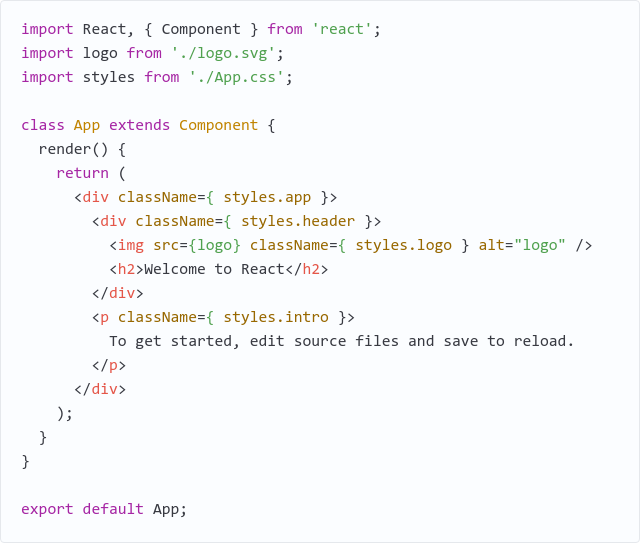
\includegraphics[height=0.4\textheight]{assets/images/theoretical2/css-module-react.png}
  \caption{Пример использования CSS модулей в React приложении}
  \label{img:cssModule__react}
\end{figure}